\documentclass[11pt]{article}
\usepackage{tikz}
\usetikzlibrary{arrows.meta,positioning}
\usepackage[margin=1in]{geometry}

\begin{document}

\section*{Exercise 4: Finite Automata}

The deterministic finite automaton in Figure~\ref{fig:dfa} accepts binary strings
whose value is divisible by three.

\begin{figure}[h]
\centering
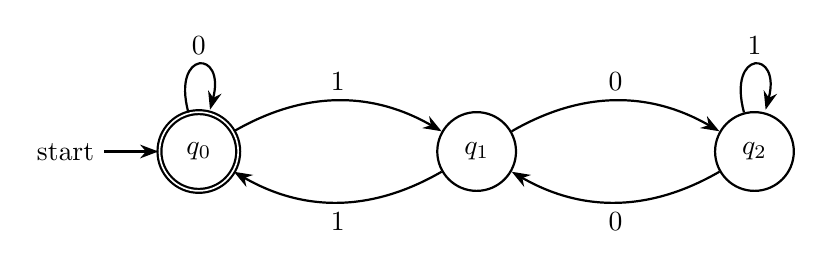
\begin{tikzpicture}[->, >=Stealth, node distance=2.5cm, thick,
                    state/.style={circle, draw, minimum size=1cm}]
  \node[state, double] (q0) {$q_0$};
  \node[state, right=of q0] (q1) {$q_1$};
  \node[state, right=of q1] (q2) {$q_2$};
  \draw (q0) edge[loop above] node {0} (q0)
        (q0) edge[bend left] node[above] {1} (q1)
        (q1) edge[bend left] node[below] {1} (q0)
        (q1) edge[bend left] node[above] {0} (q2)
        (q2) edge[bend left] node[below] {0} (q1)
        (q2) edge[loop above] node {1} (q2);
  \draw[<-] (q0) -- ++(-1.2,0) node[left] {start};
\end{tikzpicture}
\caption{DFA for multiples of three.}
\label{fig:dfa}
\end{figure}

\paragraph{Why it works.} State $q_i$ means the prefix read so far has value $\equiv i
\pmod 3$. Reading bit $b$ maps value $n$ to $2n+b$, so from $q_i$ we move to
$q_{(2i+b)\bmod 3}$.

\section*{Exercise 5: A small binary tree}

\begin{center}
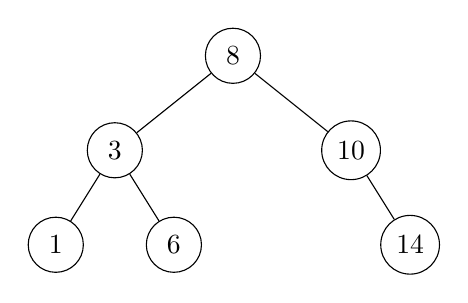
\begin{tikzpicture}[level distance=1.2cm,
  level 1/.style={sibling distance=3cm},
  level 2/.style={sibling distance=1.5cm},
  every node/.style={circle, draw, minimum size=7mm}]
  \node {8}
    child { node {3}
      child { node {1} }
      child { node {6} } }
    child { node {10}
      child[missing]
      child { node {14} } };
\end{tikzpicture}
\end{center}

An in-order traversal visits the keys in sorted order: 1, 3, 6, 8, 10, 14.

\end{document}
